This chapter introduces the elliptical PMCLP where there is no axis-parallel constraint, and the ellipses can be freely rotated. We refer to this problem as \sigla{MCER}{Planar Maximum Covering Location by Ellipses with Rotation Problem}. In comparison with MCE, this problem introduces a new variable that is responsible for determining the rotation angle of every ellipse, making MCER a more challenging problem.

\section{Definition}

An instance of the non-axis-parallel is defined exactly like the axis-parallel one on \autoref{chapter:mce}. It is given by a set of demand points $\Pp=\{p_1, \dots, p_n\}$, $p_j\in\R^2$; a list of weights $\Ww:=\{w_1, \dots, w_n\}$, with $w_j\in\R_{\ge0}$ being the weight of point $p_j$;
and $m$ ellipses given by their shape parameters $\Rr:=\{(a_1, b_1), \dots, (a_m, b_m)\}$, with $(a_j, b_j)\in\R_{>0}^2$ and $a_j>b_j$.
Additionally, to make the text more clear, we define a set of $m$ functions that represent the coverage regions of each ellipse as $\E = \{E_1, \dots, E_m\}$, with $E_j\colon \R^2\times\R \mapsto \R^2$ being a function that takes the center and angle of rotation where the $j$-th ellipse is located as input, and returns its coverage region as defined by \autoref{eq:rotated_ellipse_co}.
Lastly, an instance of MCER is defined as the tuple $(\Pp, \Ww, \Rr)$.

Given an instance of $MCER$, we define $Q:=((q_1,\theta_1); \dots; (q_m, \theta_m)) \in (\R^{2}\times[0, \pi))^m$, $(q_j, \theta_j)$ being $j$-th ellipse's the center and the angle of rotation. Then, we define MCER as the problem of determining $Q$ (placing and rotating each ellipse) to maximize the weight of the points covered by the $m$ ellipses given by
\begin{equation}\label{eq:optMCEn}
\max_{Q}{w\left(\bigcup_{i=1}^{m} \Pp \cap E_i(q_i, \theta_i)\right)}.
\end{equation}
In addition to that, we define an equivalence relation between solutions of MCER. We say that two solutions are equivalent if the set of points covered by them is the same. That is, two solutions of MCER $Q$ and $Q'$ are said to be equivalent if, and only if 
$$\bigcup_{j=1}^m\Pp \cap E_j(q_j', \theta_j') = \bigcup_{j=1}^m\Pp \cap E_j(q_j, \theta_j).$$

We also define a partial order relation between two solutions. Let $Q$ and $Q'$ be two solutions of MCER, then $Q \succ Q'$ if, and only if

$$\bigcup_{j=1}^m\Pp \cap E_j(q_j', \theta_j') \subset \bigcup_{j=1}^m\Pp \cap E_j(q_j, \theta_j).$$

In some cases, it will be more convenient to work with the one-facility version of MCER. When that is the case, we use an adapted notation removing all the unnecessary indexes, sequences and sets used to specify multiple facilities. For example, a solution of the one-facility MCER is defined as $Q := (q, \theta)$.

In the next section we present some results which ultimately lead up to the construction of a finite set that contains at least one optimal solution for MCER.

\section{An optimal and finite set of solutions}

In this section, we construct a finite list of centers and angles of rotation, also referred to as a \sigla{CLS}{Candidate Locations Set}, for each ellipse and show that at least one optimal solution is in the set of solutions created from those lists. The results presented in this section are strongly based on \autoref{chapter:e3p}, more specifically on \autoref{lema:e3p}, which states that there exists at most six solutions for any instance of E3P.

We start by introducing a lemma, which says that given an optimal solution of MCER, it is always possible to find an equivalent one, such that every ellipse covering more than one point contains two of them.

\begin{lema}\label{lema:mce_2b}
	Let $Q$ be a solution for the one-facility MCER, such that $|\Pp \cap E(q, \theta)| \ge 2$.
	There exists a solution $Q'$, such that $Q' \succ Q$ and $|\Pp \cap \partial E(q', \theta')|\ge 2$.
\end{lema}

\begin{proof}
	If we rotate the coordinate system by $-\theta$, we get a solution where the ellipse is axis-parallel.

	As it was shown in \autoref{chapter:mcd2}, $X$ is a region that is limited by arcs of ellipses. As this region is the non-empty intersection of more than one ellipse, there are at least two of these arcs that encounter at one point, creating a vertex. Selecting any of these vertices as $q'$ and $\theta'=\theta$ will make $|\Pp \cap \partial E(q', \theta')| \ge 2$.
	
\end{proof}

What \autoref{lema:mce_2b} states is that transforming any optimal solution of MCER into an equivalent optimal solution where every ellipse that covers more than one point contains two points is possible (an example can be seen in \autoref{fig:ellipse-2-points}). \autoref{lema:mce_2b} also states that this equivalent optimal solution can always be achieved by just translating the ellipses; that is, no change in the angle of rotation is required. 

\begin{figure}
	\centering
	\caption{An optimal solution before and after applying \autoref{lema:mce_2b}.}
	\includegraphics[scale=.28]{tex/figures/ellipse-2-points}
	\fautor
	\label{fig:ellipse-2-points}
\end{figure}

%Next, we define, for an optimal solution, a set of equivalent solutions, such that any ellipse covering more than one point contains at least two points.

%\begin{definicao}
%	Let $(Q^*, \Theta^*)$ be an optimal solution for an instance $(\Pp, \Ww, \Rr)$ of MCER. We define $\Pi(Q^*, \Theta^*)$ as the set of every equivalent solution of $(Q^*, \Theta^*)$, such that for any $(Q, \Theta)\in\Pi(Q^*, \Theta^*)$, for $j\in\{1, \dots, m\}$ with $|\Pp \cap E_j(q_j^*, \theta_j^*)|\ge2$, we have $|\Pp \cap \partial E_j(q_j', \theta_j)| \ge 2$.
%\end{definicao}

Next, we introduce a notation that helps us characterize angles which given an ellipse rotated by it and two points, it is possible to find a center for the ellipse, such that it contains both points.

\begin{definicao}\label{def:feasible_angle}
	Let $E$ be the coverage region of an ellipse and $u, v \in \R^2$. An angle $\theta \in [0, \pi)$ is said to be $(E, u, v)$-feasible if there is $q \in \R^2$ such that $\{u, v\} \subset \partial E(q, \theta)$.
	In addition to that, the set of $(E, u, v)$-feasible angles is referred to as 
	
	\begin{equation}
	\Phi(u, v) := \{\theta \in [0, \pi) : \theta \textnormal{ is a } (E_j,u,v)\textnormal{-feasible angle}\}.
	\end{equation}
\end{definicao}

For any $x\in\R^2$, we denote by $\angle x\in [0, \pi)$ the minimal angle between $x$ and the vector $(1, 0)$. If $\Phi(u,v)\neq\emptyset$, then $\angle(u-v)\in  \Phi(u,v)$ as $\angle(u-v)$ is the angle that makes the ellipse's major-axis, the longest segment crossing an ellipse, be parallel to the line that passes through $u$ and $v$.

In \autoref{fig:feasible-angle} two examples for \autoref{def:feasible_angle} are shown. The example with a solid border shows two given points on two different ellipses rotated by $\pi/4$, making $\pi/4$ a $(E, u, v)$-feasible angle.
The other example, with a dashed border, presents a case where the two points cannot be on the ellipse rotated by $\pi/2$, no matter where it is placed; because of that, $\pi/2$ is said to be a non $(E, u, v)$-feasible angle.

\begin{figure}[H]
	\centering
	\caption{A $(E, u, v)$-feasible angle and a not $(E, u, v)$-feasible angle.}
	\includegraphics[scale=.28]{tex/figures/feasible-angle2}
	\fautor
	\label{fig:feasible-angle}
\end{figure}

Next we open a parenthesis to discuss the problem of deciding for what angles of rotation it is possible to find a center for an ellipse, so it contains two given points. We give the result for two points that have the same $y$-coordinate, but this can be generalized.

\begin{lema}\label{lema:l-function}
	Given an instance of the one-facility MCER, if $u, v \in \Pp$ have the same $y$-coordinate and $||u-v||_2 \le 2a$, then $\Phi(u,v) = [0, \alpha] \cup [\pi - \alpha, \pi)$, for some $\alpha \in [0, \pi/2]$.
\end{lema}

\begin{proof}
	
	In \autoref{chapter:definitions}, we determined the following formula for the distance between the intersection points of an axis-parallel ellipse centered at the origin, with shape parameters $(a,b)$, and a line represented by the equation $y=mx+c$, with $m, c\in \R$:
	
	\begin{equation*}\label{eq:dist_line_ellipse}
	D(m, c)=\dfrac{\sqrt{(a^2m^2+b^2-c^2)(4a^2b^2(1+m^2))}}{(a^2m^2+b^2)},
	\end{equation*}
	with $D : \R^2 \mapsto \R_{\ge0}$ being a function of the line parameters $(m, c)$.
	If $D(m, c) = ||u-v||_2$, then there exists $q_1, q_2 \in \R^2$, such that $\{u, v\} \subset \partial E(q_1, \tan{m})$ and $\{u, v\} \subset \partial E(q_2, \pi-\tan{m})$. It is also possible to see that, when $m$ is fixed, $D(m, c)^2$ is a parabola, and that $D(m, c)$ is maximized at $c=0$.  
	Following that, we define a function $L:\R\mapsto\R$ as
	
	\begin{equation*}
	L(m):= D(m, 0)^2 = \dfrac{(a^2m^2+b^2)(4a^2b^2(1+m^2))}{(a^2m^2+b^2)^2},
	\end{equation*}
	which describes the maximum distance between points of an ellipse-line intersection considering all lines with $m$ angular coefficient. 
	An example of that function is shown in \autoref{fig:L-function-plot}.	
	From that, if $L(m) \ge ||v-u||_2^2$, then there exists $q_1, q_2\in\R^2$, such that $\{u, v\} \subset \partial E(q_1, \tan{m})$, and $\{u, v\} \subset \partial E(q_2, \pi-\tan{m})$.
	
	It is possible, by calculating the derivatives, to conclude that $L$ has its maximum at $m=0$, is increasing in $[0, \infty)$, is decreasing in $(-\infty, 0]$, and attains every value in the interval $(4b^2, 4a^2]$. Notice that $L$ never hits $4b^2$ because that is the distance between the intersection of the ellipse with a vertical line.
	%In \autoref{fig:L-function-plot}, an example of function $L$ is shown with $(a, b) = (2, 1)$.
	
	If $\inf{L} \ge ||u-v||_2^2$, then $\Phi(u,v) = [0, \pi)$.
	Otherwise, let $\beta \in \R$, $\beta \ge 0$, such that $L(\beta) = ||u-v||_2^2$, then as $m>\beta$, we have $L(m) < ||u-v||_2^2$, which means that it is impossible to make the ellipse contain $u$, and $v$.
	As $L$ is an even function, the same can be said for $m < \beta$. Therefore, we conclude that $\Phi(u,v)=[0, \tan(\beta)] \cup [\pi-\tan(\beta), \pi)$.
\end{proof}

\begin{figure}[H]
	\centering

	\caption{Plot of function $L$ in the interval $[-7, 7]$.}
	\includegraphics[scale=.4]{tex/figures/L-function-plot}
	\fautor
	\label{fig:L-function-plot}
\end{figure}

Following that, we introduce a lemma that is responsible for connecting the developments of this chapter with the results of \autoref{chapter:e3p}.
This lemma makes it possible to describe a type of solution which, for sure, is part of the equivalence class of any optimal solution.
It states that, for any ellipse that covers more than two points in a given optimal solution, an equivalent solution exists with at least one of the two properties:
\begin{itemize}
	\item The ellipse contains at least three points.
	\item The ellipse contains two points for any feasible angle.
\end{itemize}

\begin{lema}\label{lema:3pnts}
Let $Q^*$ be a solution of the one-facility MCER, such that $|\Pp \cap E(q^*, \theta^*)|\ge2$.
If for all $\bar{Q} \succ Q^*$, $|\Pp \cap \partial E(\bar{q}, \bar{\theta})| < 3$, then there exists $\{u, v\} \subset \Pp \cap E(q^*, \theta^*)$, such that for all $\theta\in \Phi(u,v)$ there exists $q \in \R^2$, such that $(q, \theta)$ is equivalent to $Q^*$.

\end{lema}

\begin{proof}
	According to \autoref{lema:mce_2b}, there exists $\{u, v\} \subset \Pp \cap E(q^*, \theta^*)$, such that $Q' \succ Q^*$ exists, and $\{u, v\} \subset \partial E(q', \theta^*)$. Therefore, $\theta^*\in\Phi(u,v)$.
	
	Suppose that $u$ and $v$ have the same $y$-coordinate (if they do not, a rotation can be applied to make them do). Then, by \autoref{lema:l-function}, $\Phi(u,v)=[0, \alpha] \cup [\pi-\alpha, \pi)$, for some $\alpha \in [0, \pi/2]$. Then, if we rotate the coordinate system by $\pi-\alpha$, we obtain $\Phi(u,v)=[0, 2\alpha]$.
	
	With this result in hand, we can use a continuity argument to complete our proof as follows.
	Let $\delta : \Phi(u,v) \mapsto \R^2$ be a continuous function which takes an angle $\theta\in\Phi(u,v)$ and returns a center, such that $\{u,v\} \subset \partial E(\delta(\theta), \theta)$, and, from solution $Q'$, $\delta(\theta') = q'$. Notice that, in general, for any angle in $\Phi(u,v)$, there are two possible centers that make $\{u,v\} \subset \partial E(\delta(\theta), \theta)$ (see \autoref{fig:feasible-angle} for an example), however, imposing $\delta(\theta') = q'$ makes $\delta$ be a well-defined continuous function. This is shown in \autoref{fig:lema-3-points} where $\delta$ is plotted for the whole interval $\Phi(u,v)$.
	
	Let $w\in \Pp \setminus \{u,v\}$, then we define $f_w  : [0, \pi) \mapsto \R_{\ge0}$ to be a function that takes an angle of rotation $\theta$ and returns the elliptical distance $||\cdot||_{a,b,\theta}$ to the center $\delta(\theta)$; that is $f_w(\theta)=||w-\delta(\theta)||_{a,b,\theta}$.
	We have that if $w \in \Pp \cap E(q^*, \theta^*)$, then $f_w(\theta^*) \le 1$; and if $w \not\in \Pp \cap E(q^*, \theta^*)$, then $f_w(\theta^*) > 1$.
	
	Therefore, if there exists $\theta\in\Phi(u,v)$, such that for all $q\in\R^2$, $(q, \theta)$ is not equivalent to $Q^*$, then there exists either $w \in \Pp \cap E(q^*, \theta^*)$, with $f_w(\theta)>1$, or $w \not\in \Pp \cap E(q^*, \theta^*)$, with $f_w(\theta)\le 1$. Because $f_w$ is continuous, there exists $\bar{\theta}\in\Phi(u,v)$, such that $f_w(\theta)=1$, implying that $|\Pp \cap \partial E(\delta(\bar{\theta}), \bar{\theta})| \ge 3$.
\end{proof}

%\begin{figure}[H]%
%	\centering%
%	\caption{Every ellipse that contains two points for a fixed angle of %rotation.}
%	\includegraphics[scale=.36]{tex/figures/2point-ellipse}
%	\fautor
%	\label{fig:2point-ellipse}
%\end{figure}

What \autoref{lema:3pnts} states is that, for every ellipse in an instance of MCER, unless an equivalent optimal solution with three points on it exists, the angle of rotation can practically be ignored. Because of that, it will be shown that we can construct a CLS for each ellipse which is finite and also contains an optimal solution.

In \autoref{fig:lema-3-points}, a visualization of \autoref{lema:3pnts} is presented.
An initial optimal solution is given by the dashed-border ellipse and its center, represented by a star point. From it, the continuous function $\delta$ is defined by moving the ellipse through the rotation angles in $\Phi_j(u,v)$ while maintaining $u, v$ on it. Ten angles were chosen from $\Phi_j(u,v)$ to be shown in \autoref{fig:lema-3-points}, among those were $0$ and $\max\{\Phi_j(u,v)\}$; their corresponding ellipses are displayed with solid-line borders.
Consistently with \autoref{lema:3pnts}, the points in $\Pp \setminus \{u, v, w\}$ stay within the ellipse's cover for any angle of rotation, and, for point $w$, there exists an angle, such that it is on the ellipse.  

\begin{figure}[H]
	\centering
	\caption{A visualization of \autoref{lema:3pnts}.}
	\includegraphics[scale=.9]{tex/figures/lema-3-points}
	\fautor
	\label{fig:lema-3-points}
\end{figure}

Let $Q^*$ be any optimal solution of an instance $(\Pp, \Ww, \Rr)$ of MCER. We will define a set of solutions $\Omega$ and show that there exists an equivalent solution $Q'$ to  $Q^*$, such that $Q' \in \Omega$. This is the same thing as showing that $\Omega$ for sure contains an optimal solution for the instance $(\Pp, \Ww, \Rr)$.
Before that, we introduce a definition for the CLS of every ellipse, which is then used to construct the set of solutions $\Omega$.

\begin{definicao}\label{def:Sj}
	Given an instance of MCER. Then, for all $j\in\{1, \dots, m\}$, we define the CLS of the $j$-th ellipse as $S_j = S_j^{(1)} \cup S_j^{(2)} \cup S_j^{(3)}$ with
\begin{align*}
S_j^{(1)} &= \bigcup_{u \in \Pp} \{(u, 0)\}\\
S_j^{(2)} &= \bigcup_{\{u, v\} \subset \Pp} \{(q, \angle(u-v))\in \R^2\times[0, \pi): \{u,v\} \subset \partial E_j(q, \angle(u-v))\}\\
S_j^{(3)} &= \bigcup_{\{u, v, w\} \subset \Pp} \{(q, \theta)\in \R^2\times[0, \pi): \{u, v, w\} \subset \partial E_j(q, \theta)\}.
\end{align*}
\end{definicao}

This definition breaks the construction of the CLS into three separated cases. The first one, $S_j^{(1)}$, represents solutions where the $j$-th ellipse covers only one point. The second one, $S_j^{(2)}$, takes into account solutions where the $j$-th ellipse covers at least two points, and no equivalent solution with three points on the ellipse exists. The last case, $S_j^{(3)}$, considers solutions where there exists an equivalent one with three points on the $j$-th ellipse. 

To compute $S_j^{(2)}$, we can observe that, given two points $u, v$, determining every $q\in\R^2$, such that $\{u,v\}\subset\partial E_j(q, \angle(u-v))$ can be transformed into the problem of determining the set $\partial E_j(u, \angle(u-v)) \cap \partial E_j(v, \angle(u-v))$, which, by \autoref{lema:mce_2b}, is composed of at most two points, which can be determined analytically. Therefore, we have that $S_j^{(2)}$ can be computed in $\bigO(n^2)$ operations.

To compute $S_j^{(3)}$, we have to call \autoref{algoritmo:e3p}, which by \autoref{th:e3p} is $\bigO(1)$.

Overall, constructing every ellipse's CLS can be implemented to have a $\bigO(n^3)$ runtime complexity.
Following this, we introduce a theorem, which connects the results for MCER so far, to prove that the set of solutions constructed using the CLSs described by \autoref{def:Sj} contains an optimal solution.

\begin{theorem}\label{th:mcer}
	Given an instance of MCER, let $\Omega$ be a set of solutions defined as 
\begin{equation*}\label{eq:omega}
\Omega = \{Q \in (\R^2\times[0, \pi))^m \colon (q_j, \theta_j) \in S_j \textnormal{ for all } j\in\{1, \dots, m\}\},
\end{equation*}
Then there exists an optimal solution $Q^* \in \Omega$, and $|\Omega|\le n^{3m}$.
\end{theorem}
\begin{proof}
		The first thing to notice is that $\Omega$ is defined as the combination of every possible solution from each CLS. To prove that it contains an optimal solution $Q^*$, we only need to prove that for all $j\in\{1, \dots, m\}$, there exists $(q_j, \theta_j)\in S_j$, such that $\Pp \cap E_j(q_j^*, \theta_j^*) \subset \Pp \cap E_j(q_j, \theta_j)$. To do that, we use \autoref{lema:3pnts} and break the possible optimal solutions into three cases.
	
	In the first case, we consider solutions where the $j$-th ellipse covers less than one point, that is, $|\Pp \cap E_j(q_j^*, \theta_j^*)|\le1$. It is possible to see that $S_j^{(1)}$ takes this possibility into account as it includes in $\Omega$ every solution that has an ellipse centered at a point from $\Pp$. From that, we can also conclude that $|S_j^{(1)}| \le n$.
	
	In the second case, we consider solutions where the $j$-th ellipse covers at least two points, and there is no $Q' \succ Q^*$, such that $|\Pp \cap \partial E_j(q_j', \theta_j')| \ge 3$.
	This case is addressed by \autoref{lema:3pnts}, which states that there are equivalent solutions to $Q^*$ with two points $u, v \in \Pp \cap E_j(q_j^*, \theta_j^*)$ on the $j$-th ellipse for every $(E_j, u, v)$-feasible angle.
	As $\angle(u-v)$ is a $(E_j, u, v)$-feasible angle, we have that there exists $(q_j, \theta_j) \in S_j^{(2)}$, such that $\Pp \cap E_j(q_j, \theta_j) = \Pp \cap E_j(q_j^*, \theta_j^*)$.
	Also, by \autoref{lema:mce_2b}, we have that $|S_j^{(2)}| \le 2\binom{n}{2}$.
	
	%	Moreover, as determining every $q\in\R^2$, such that $\{u,v\}\subset \partial E_j(q, \angle(u-v))$ can be transformed into the problem of determining the set $\partial E_j(u, \angle(u-v)) \cap \partial E_j(v, \angle(u-v))$, which, as discussed in \autoref{section:mce}, contains at most two points, we can conclude that $|S_j^{(2)}| \le 2 \binom{n}{2}$.
	
	For the last case, we are left with solutions where the $j$-th ellipse covers more than two points, and there exists an equivalent solution with three points on it. 
	As $S_j^{(3)}$ contains every center and angle of rotation that puts three points on the $j$-th ellipse, an equivalent solution for this case is present in the set of solutions $\Omega$. Also, by \autoref{lema:e3p} we can conclude that $|S_j^{(3)}| \le 6\binom{n}{3}$.
	
	Combining the three cases, as $S_j=S_j^{(1)}\cup S_j^{(2)} \cup S_j^{(3)}$, we get the following bound for $|S_j|$:
	\begin{eqnarray*}
		|S_j| &\le 6\binom{n}{3} + 2\binom{n}{2} + n &= n(n-1)(n-2) + n(n-1) + n\\
		|S_j| &\le 6\binom{n}{3} + 2\binom{n}{2} + n &= n((n-1)^2+1) \le n^3.
	\end{eqnarray*}	
	Therefore, we conclude that  $|\Omega| \le |S_1|\times \dots \times |S_m| \le n^{3m}$.
\end{proof}


\section{An algorithm for MCER}

In this section we describe an algorithm for MCER that does a complete search on the CLS of each ellipse.
Firstly, in \autoref{algoritmo:mcer1}, we present a procedure called CLS-MCER which returns the CLS for an ellipse with shape parameters $(a, b)$. Then, in \autoref{algoritmo:mcer} we describe the procedure that returns an optimal solution for MCER.

Let $E$ be the coverage region of an ellipse with shape parameters $(a, b)$. We assume that in \autoref{algoritmo:mcer1}, the procedure $e2p(u, v, a, b)$ returns every $(q, \angle(u-v) \in \R^2\times[0, \pi)$, such that, $\{u, v\}\subset \partial E(q, \angle(u-v))$. That is, this procedure returns every location for the ellipse with shape parameters $(a, b)$, such that its angle of rotation is $\angle(u-v)$, and the points $u$, $v$ are on the ellipse. This can be done using the results of Section~\ref{section:ellipses_intersection2}.

\begin{algoritmo}
	\caption{Algorithm that constructs a CLS for an ellipse.}\label{algoritmo:mcer1}
	\begin{algorithmic}[1]
		\Require{A set of points $\Pp=\{p_1,\dots,p_n\}$, and an ellipse's shape parameters $(a, b)$.}
		
		\Ensure{A CLS for the ellipse with shape parameters $(a, b)$ considering the demand set $\Pp$.}
		
		\item[]
		
		\Procedure{CLS-MCER}{$\Pp, a, b$}
		\State $S \gets \{\}$
		
		\For {$u \in \Pp$}
		\State $S \gets S \cup \{(u, 0)\}$
		\EndFor
		
		\For {$\{u, v\} \in \Pp$}
		\State $S \gets S \cup e2p(u, v, a, b)$
		\EndFor
		
		\For{$\{u, v, w\} \in \Pp$}
		\State $S \gets S \cup e3p(u, v, a, b)$ \Comment{Defined in \autoref{algoritmo:e3p}.}
		\EndFor
		
		\State \Return $S$
		\EndProcedure
	\end{algorithmic}
\end{algoritmo}

After that, we define \autoref{algoritmo:mcer} which takes an instance $(\Pp, \Ww, \Rr)$ of MCER, and returns an optimal solution for it.
Even though it is based on \autoref{th:mcer}, the set of solutions $\Omega(\Pp, \Ww, \Rr)$ is not explicitly built in \autoref{algoritmo:mcer}. Instead, a complete search is done by backtracking the CLS of every ellipse returned by procedure CLS-MCER defined in \autoref{algoritmo:mcer1}.

Two procedures are defined in \autoref{algoritmo:mcer}. The first one, called $MCER$, returns an optimal solution for an instance $(\Pp, \Ww, \Rr)$ using the second procedure $MCER_{bt}$. This second procedure is responsible for the backtracking and takes two additional parameters $j\in\{1, \dots, m\}$, which represents the index of the ellipse that $MCER_{bt}$ is currently processing, and $Z\subset \Pp$, which represents the set of points that have not been covered by the ellipses with indexes $1, \dots, j-1$.


\begin{algoritmo}
	\caption{Algorithm for MCER}\label{algoritmo:mcer}
	\begin{algorithmic}[1]
		\Require{A set of points $\Pp=\{p_1,\dots,p_n\}$, a list of weights $\Ww=\{w_1, \dots, w_n\}$, and a list of shape parameters $\Rr=\{(a_1, b_1), \dots, (a_m, b_m)\}$.}
		
		\Ensure{An optimal solution for the given instance of MCER.}
		
		\item[]
		\Procedure{$MCER$}{$\Pp, \Ww, \Rr$}
		\State \Return $MCER_{bt}(\Pp, \Ww, \Rr, 1)$
		\EndProcedure
		
		\item[]
		
		\Procedure{$MCER_{bt}$}{$Z, \Ww, \Rr, j$}
		%\If{$j = m+1$}
		%\State \Return $0$
		%\EndIf
		
		%\State $ans \gets 0$
		\State $(q_{j}^*, \dots, q_m^*); (\theta_{j}^*, \dots, \theta_m^*) \gets (0, \dots 0); (0, \dots, 0)$ \Comment{Setting to $0$ as a default value.}
		
		\State $S_j \gets \textnormal{CLS-MCER}(Z, a_j, b_j)$

		
		\ForAll{$(q_j, \theta_j) \in S_j$}
		%\State $Cov \gets \Pp \cap E_j(q_j, \theta_j)$
		
		\If{$j < m$}
		\State $(q_{j+1}, \dots, q_m); (\theta_{j+1}, \dots, \theta_m) \gets  MCER_{bt}(Z\setminus Cov, \Ww, \Rr, j+1)$
		\EndIf
		
		%\State $Cov \gets \bigcup_{k=j}^m \Pp \cap E_k(q_k, \theta_k)$
		\If {$w(\bigcup_{k=j}^m \Pp \cap E_k(q_k, \theta_k)) > w(\bigcup_{k=j}^m \Pp \cap E_k(q_k^*, \theta_k^*))$}
			%\State $ans \gets w(Cov)$
			%\State $((q_{j}^*,\theta_{j}^*); \dots; (q_m^*, \theta_m^*)) \gets ((q_{j},\theta_{j}); \dots; (q_m, \theta_m))$
			
			\State $(q_{j}^*, \dots, q_m^*); (\theta_{j}^*, \dots, \theta_m^*) \gets (q_{j}, \dots, q_m); (\theta_{j}, \dots, \theta_m)$
		\EndIf
		\EndFor
		
		\State \Return $(q_{j}^*, \dots, q_m^*); (\theta_{j}^*, \dots, \theta_m^*)$
		\EndProcedure
	\end{algorithmic}
\end{algoritmo}

\begin{corolario}
	\autoref{algoritmo:mcer} takes $\bigO(mn^{3m+1})$ operations and returns an optimal solution for an instance of MCER.
\end{corolario}

\begin{proof}
	For every $j\in\{1, \dots, m\}$, unless $Z=\{\}$, when choosing the center and angle of rotation for the $j$-th ellipse, \autoref{algoritmo:mcer} does not consider any $(q_j, \theta_j) \in \R^2 \times \R$, such that $Z \cap E_j(q_j, \theta_j) = \{\}$. Apart from those solutions, which are non-optimal, \autoref{algoritmo:mcer} considers every solution in $\Omega$. As evaluating each solution can be done in $\bigO(nm)$, we get the overall runtime complexity of $\bigO(mn^{3m+1})$.
\end{proof}

In \autoref{fig:AB120}, a solution returned by \autoref{algoritmo:mcer} for the instance AB120 taken from \citeonline{andreta} is displayed. The exact method developed by \citeonline{andreta}, for this instance, could not obtain an optimal solution within the established time limit, however, comparing with the solution obtained by our algorithm, their heuristic method does find an optimal solution. In the next chapter, we give more details about the solutions found by our algorithm, along with the proposal of some new instances for MCER.


\begin{figure}[!htb]
	\centering
	\caption{An optimal solution of MCER-$k$ for the instance AB120.}
	\includegraphics[scale=.8]{tex/figures/AB120}
	\fautor
	\label{fig:AB120}
\end{figure}

\subsection{Adding facility cost}

In this section, we consider the extended version of MCER where each facility has a cost assigned to it and exactly $k$ of them must be used in a solution. We refer to this version of the problem as \sigla{MCER-$k$}{Maximum Covering by Ellipses with Rotation and a $k$-constraint}. 

An instance of MCER-$k$ has the same parameters as MCER plus a list of costs \mbox{$\Cc:=\{c_1, \dots, c_m\}$}, with $c_j\in\R_{>0}$ being the cost of the $j$-th facility; and $k\in\mathbb{N}$, $k\le m$.

A solution for MCER-$k$ is given by $(I, Q, \Theta)$, with $I:=\{i_1, \dots, i_k\}\subset \{1, \dots, m\}$; \\\mbox{$Q:=(q_1, \dots, q_k)\in\R^{2k}$}, with $q_j$ being the center of the $i_j$-th ellipse; and \mbox{$\Theta:=(\theta_1, \dots, \theta_k) \in [0, \pi)^k$}, with $\theta_j$ being the angle of rotation of the $i_j$-th ellipse. An optimal solution of MCER-$k$ is given by the optimization problem

\begin{equation*}
	\max_{I, Q, \Theta} w\left(\bigcup_{j=1}^k \Pp \cap E_{i_j}(q_j, \theta_j)\right).
\end{equation*}

Then, in the same way that it is done in \autoref{chapter:mcd2}, we introduce \autoref{algoritmo:mcer-k} for MCER-$k$ that uses \autoref{algoritmo:mcer} for every $I:=\{i_1, \dots, i_k\} \subset \{1, \dots, m\}$. Therefore, \autoref{algoritmo:mcer-k} returns an optimal solution for MCER-$k$ in $\bigO(k\binom{m}{k}n^{3k+1}) = \bigO(m2^mn^{3m+1})$ time.

\begin{algoritmo}
	\caption{Algorithm for MCER-$k$}\label{algoritmo:mcer-k}
	
	
	\begin{algorithmic}[1]
		\Require{A set of points $\Pp=\{p_1,\dots,p_n\}$, a list of weights $\Ww=\{w_1, \dots, w_n\}$, a list of shape parameters $\Rr=\{(a_1, b_1), \dots, (a_m, b_m)\}$, a list of costs $\Cc=\{c_1, \dots, c_m\}$, and $k\in \mathbb{N}$.}
		\Ensure{An optimal solution for MCER-$k$.}
		
		\item[]
		
		\Procedure{MCER-$k$}{$\Pp, \Ww, \Rr, \Cc, k$}
		\State $I^* = \{i_1^*, \dots, i_k^*\}\gets \{1, \dots, k\}$
		\State $Q^* = (q_1^*, \dots, q_k^*) \gets (0, \dots, 0)$
		\State $\Theta^* = (\theta_1^*, \dots, \theta_k^*) \gets (0, \dots, 0)$
		
		\ForAll{$I=\{i_1, \dots, i_k\} \subset \{1, \dots, m\}$}
		
		\State $\Rr' \gets \{(a_j, b_j) \in \Rr: j \in I\}$
		\State $(q_1, \dots, q_k); (\theta_1, \dots, \theta_k) \gets MCER(\Pp, \Ww, \Rr')$
		
		\If{$w(\bigcup_{j=1}^k \Pp \cap E_{i_j}(q_j, \theta_j)) - \sum_{j\in I} c_j > w(\bigcup_{j=1}^k \Pp \cap E_{i_j^*}(q_j^*, \theta_j^*)) - \sum_{j\in I^*}c_{j}$}
		\State $Q^* \gets (q_1, \dots, q_k)$
		\State $\Theta^* \gets (\theta_1, \dots, \theta_k)$
		\State $I^* \gets I$
		\EndIf
		\EndFor
		
		\State \Return $I^*, Q^*, \Theta^*$
		\EndProcedure
	\end{algorithmic}
\end{algoritmo}